\documentclass{standalone}
\usepackage{tikz}
\usepackage{ctex,siunitx}
\setCJKmainfont{Noto Serif CJK SC}
\usepackage{tkz-euclide}
\usepackage{amsmath,bbding}
\usetikzlibrary{patterns, calc}
\usetikzlibrary {decorations.pathmorphing, decorations.pathreplacing, decorations.shapes,}

\begin{document}
\small
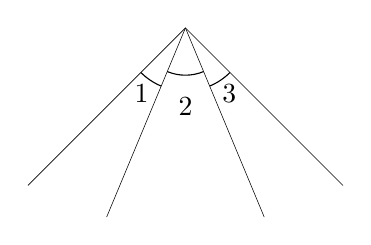
\begin{tikzpicture}[>=stealth,scale=2]
  \tkzSetUpPoint[fill=black]
  % \useasboundingbox(-0.1,-2.5)rectangle(6,3);
	\tkzDefPoints{0/.5/O, -1/-.5/A, -.5/-.7/B, .5/-.7/C, 1/-.5/D}
	\tkzDrawSegments(O,A O,B O,C O,D)
	\tkzMarkAngles[mark=none, size=.4](A,O,B C,O,D)
	\tkzLabelAngle[pos=.5](A,O,B){1}
	\tkzLabelAngle[pos=.5](B,O,C){2}
	\tkzLabelAngle[pos=.5](C,O,D){3}
	\tkzMarkAngles[mark=none, size=.3](B,O,C)
\end{tikzpicture}
\end{document}